\documentclass[11pt,twocolumn,twoside,lineno]{pnas-new}
% Use the lineno option to display guide line numbers if required.
\usepackage{noto}

\templatetype{pnasresearcharticle} % Choose template 
% {pnasresearcharticle} = Template for a two-column research article
% {pnasmathematics} %= Template for a one-column mathematics article
% {pnasinvited} %= Template for a PNAS invited submission

\title{The LQR Controller}

% Use letters for affiliations, numbers to show equal authorship (if applicable) and to indicate the corresponding author
\author[a,b]{\href{https://github.com/sezer-muhammed?tab=repositories}{Muhammed Sezer}}
\author[a,b]{Şevval Belkıs Dikkaya} 

\affil[a]{\href{https://www.metu.edu.tr/}{Middle East Technical University}}
\affil[b]{\href{https://www.orionrobotics.org}{Orion Robotics Ltd.}}

% Please give the surname of the lead author for the running footer
\leadauthor{Sezer} 

% Please add here a significance statement to explain the relevance of your work
\significancestatement{This document's significance lies in its comprehensive exploration of the Linear Quadratic Regulator (LQR) controller, a key tool in the realm of system control.}

% Please include corresponding author, author contribution and author declaration information
\equalauthors{\textsuperscript{1}Muhammed Sezer and Şevval Dikkaya contributed equally to this work.}
\correspondingauthor{\textsuperscript{2}To whom correspondence should be addressed. E-mail: muhammedsezer12@gmail.com}

% Keywords are not mandatory, but authors are strongly encouraged to provide them. If provided, please include two to five keywords, separated by the pipe symbol, e.g:
\keywords{Linear Quadratic Regulator $|$ LQR $|$ Control Theory $|$ System Control $|$ Practical Application $|$ Simulation $|$ Performance Analysis $|$ Case Study}


\begin{abstract}
       In this easy-to-follow guide on the Linear Quadratic Regulator (LQR) controller, you'll learn about its practical and theoretical aspects. It equips you with the knowledge to not only run simulations but also to apply it in real-world scenarios. From understanding the underlying principles to discussing practical applications, and even a step-by-step demonstration via a computer simulation, this guide covers it all. Whether you're a beginner or an experienced practitioner, this guide aims to give you a complete picture of the LQR controller, and how it can be a game-changer in tackling complex control problems.
\end{abstract}

\dates{\today}

\begin{document}

\maketitle
\thispagestyle{firststyle}
\ifthenelse{\boolean{shortarticle}}{\ifthenelse{\boolean{singlecolumn}}{\abscontentformatted}{\abscontent}}{}


\section{Introduction}
\subsection{Overview of LQR}

Once upon a time, in the mid-20th century, the field of control systems was undergoing a revolution. Engineers and mathematicians were seeking new ways to manage complex, dynamic systems. Amidst this backdrop, the Linear Quadratic Regulator (LQR) was born, a brainchild of the need for optimal control strategies.

The LQR was first introduced in the 1960s, during a period of rapid advancement in aerospace technology. The space race was in full swing, and the need for precise, reliable control systems for spacecraft was paramount. The traditional methods of control system design were not sufficient for these high-stakes, complex tasks. The world needed a new approach, and the LQR provided just that.

The LQR was a game-changer. It provided a systematic, principled approach to control system design. By defining a cost function that quantified the trade-off between system performance and control effort, and then minimizing this cost function, the LQR could determine the optimal control law for a given system.

Over the years, the LQR has proven its worth in a wide range of applications, from aerospace and robotics to economics and beyond. It is particularly well-suited for systems that can be accurately modeled by linear equations, and where the cost to be minimized can be expressed as a quadratic function. However, even for non-linear systems, LQR can often provide useful results when applied to a linear approximation of the system around a particular operating point.

In the following sections, we will delve deeper into the story of LQR, its applications, and its implementation. We will start with a specific problem, then introduce the LQR as a solution, and finally explore the theory behind it. We will also discuss how to implement an LQR solution and analyze the results of a simulation. So, buckle up and get ready for an exciting journey into the world of LQR!

\subsection{Importance and Applications of LQR}
The Linear Quadratic Regulator (LQR) has been a cornerstone in the field of control systems engineering due to its systematic and optimal approach to control system design. Its ability to balance system performance against control effort has made it a valuable tool across a multitude of industries.

The parameters used in LQR control design are primarily the weights in the quadratic cost function. These weights are chosen based on the specific requirements of the system being controlled. They reflect the relative importance of achieving a particular system state versus the amount of control effort expended.

Let's delve into some specific applications and the parameters typically used:

\begin{enumerate}
       \item \textbf{Aerospace}: In the design of control systems for aircraft and spacecraft, the cost function might be weighted more heavily towards achieving a specific altitude or speed (system state), with less weight given to control effort. This is because precise control is often critical in these applications.
       \item \textbf{Automotive}: In applications like cruise control systems and active suspension systems, the cost function might be weighted to balance ride comfort (a function of the vehicle's state) and fuel efficiency (a function of the control effort).
       \item \textbf{Robotics}: In controlling robotic arms, unmanned aerial vehicles (drones), and autonomous vehicles, the weights in the cost function might be chosen to balance the precision of the task execution (system state) and energy efficiency (control effort).
       \item \textbf{Energy Sector}: In optimizing the operation of power systems, such as power plants and electrical grids, the cost function might be weighted more heavily towards maintaining a stable power output (system state), with less weight given to the cost of operation (control effort).
       \item \textbf{Economics}: In dynamic optimization problems, such as maximizing economic output while minimizing costs, the weights in the cost function would reflect the relative importance of these two factors.
\end{enumerate}

In each of these applications, the specific weights used in the LQR design would depend on the specific requirements and constraints of the system and the task at hand. As we delve deeper into the theory and implementation of LQR in the following sections, you will gain a deeper understanding of how these parameters are chosen and how they influence the performance of the LQR controller.

\subsection{Prerequisites and Assumptions}
Before we dive deeper into the world of Linear Quadratic Regulator (LQR), it's important to understand the prerequisites and assumptions that underpin this control strategy. This will ensure that we have a solid foundation upon which to build our understanding of LQR.

\subsubsection{Prerequisites:}
Knowledge in the following areas is assumed for this course:

\begin{itemize}
       \item \textbf{Linear Algebra}: Understanding of matrices, vectors, and operations on them is essential as the state-space representation of systems, which is central to LQR, is expressed in matrix form.
       \item \textbf{Differential Equations}: Familiarity with ordinary differential equations is crucial as the dynamics of the systems we'll be controlling are often expressed as such equations.
       \item \textbf{Control Systems}: Basic understanding of control systems, particularly state-space representation of systems, is required. This includes knowledge of system dynamics, stability, and controllability.
       \item \textbf{Laplace Transforms}: Familiarity with Laplace transforms is helpful for understanding the analysis and design of control systems.
\end{itemize}

\subsubsection{Assumptions:}
When working with LQR, we typically make the following assumptions:

\begin{itemize}
       \item \textbf{Linearity}: The system to be controlled is assumed to be linear, or at least well-approximated by a linear model around the operating point of interest.
       \item \textbf{Quadratic Cost Function}: We assume that the cost to be minimized can be expressed as a quadratic function of the system states and control inputs.
       \item \textbf{Full State Accessibility}: We assume that all states of the system are measurable and available for feedback. If this is not the case, techniques such as state estimation may be required.
       \item \textbf{Deterministic System}: We assume that the system is deterministic, i.e., there are no random disturbances affecting the system. If such disturbances are present, a different approach, such as stochastic control, may be more appropriate.
\end{itemize}

With these prerequisites and assumptions in mind, we are now ready to embark on our journey into the fascinating world of LQR.


\section{Example Problem}
\subsection{Problem Statement: The Inverted Pendulum}
Our challenge is the inverted pendulum problem, a topic that has intrigued researchers from the past to the present. With its canonical and nonlinear structure, the inverted pendulum problem has been a popular subject for control theories and applications.

The inverted pendulum problem comes in various forms: the cart-pole inverted pendulum, the double pendulum cart-pole, the rotary inverted pendulum, and the mobile inverted pendulum. The balancing problems of these systems are widely covered in the literature and are still relevant today.

In this study, realized with a different approach to the balance problem of the inverted pendulum, the nonlinear mathematical model of the pendulum is linearized, and control is performed with full state feedback. When designing the controller, the goal is to keep the pendulum balanced vertically and bring the cart back to the starting point. You can see the pendulum system at figure \ref{pendulum}
\begin{figure}[h]
       \centering
       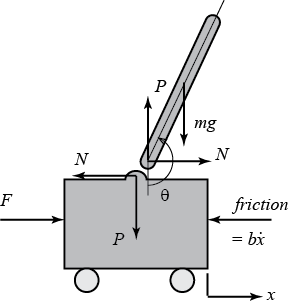
\includegraphics[width=0.9\linewidth]{problem/pendulum.png}
       \caption{Inverted Pendulum System}
       \label{pendulum}
\end{figure}

\subsection{Problem Analysis}
The inverted pendulum problem is a classic in control theory due to its inherently unstable nature. It's a classic example of an unstable system that requires active control to maintain its equilibrium state. 

The system consists of a cart of mass M that can move horizontally and a pendulum of length l and mass m attached to the cart. The pendulum is free to rotate and its angle with the vertical, denoted by $\theta$, is a critical parameter. The pendulum is in its unstable equilibrium position when $\theta$ is 180 degrees, i.e., when it's perfectly vertical. 

The control input to the system is a force F applied horizontally to the cart. The goal is to adjust this force to keep the pendulum upright, i.e., to keep $\theta$ as close to 180 degrees as possible. 

However, the system is nonlinear and underactuated, meaning it has more degrees of freedom (two, in this case: the position of the cart and the angle of the pendulum) than it has independent control inputs (one, in this case: the force applied to the cart). This makes the control problem challenging.

Moreover, the system is highly sensitive to disturbances and changes in the initial conditions. A small push to the pendulum or a small change in the initial angle can cause the pendulum to fall over. 

In the next section, we will define the specific goals and objectives for the control problem.



\subsection{Goals and Objectives}
In this section, we will define the specific goals and objectives for the control of the inverted pendulum system. Our aim is to control both the pendulum's angle $\theta$ and the cart's position $x$.

To ensure the performance of our system, we need to set some quantitative requirements. These requirements will serve as our definition of a "good" system. In control theory, we often use specific performance measures to define these requirements. For our inverted pendulum system, we will focus on the following performance measures:

\begin{itemize}
    \item \textbf{Settling Time}: This is the time it takes for the system to converge to its desired final state. For our system, we want the cart to reach its commanded position and the pendulum to reach its vertical position within 5 seconds.
    \item \textbf{Rise Time}: This is the time it takes for the system to go from its initial state to its desired final state for the first time. For our system, we want the cart to reach its commanded position for the first time in less than 0.5 seconds.
    \item \textbf{Overshoot}: This is the extent to which the system exceeds its desired final state. For our system, we want the pendulum angle $\theta$ to never deviate more than 20 degrees (0.35 radians) from the vertical position.
    \item \textbf{Steady-State Error}: This is the difference between the desired final state and the actual final state that the system reaches after a long time. For our system, we want the steady-state error to be less than 2\% for both $x$ and $\theta$.
\end{itemize}

In summary, our goal is to design a controller that can meet these performance requirements, effectively balancing the pendulum in its upright position while controlling the position of the cart.


\section{Solution! LQR}
\subsection{Introduction to LQR as a Solution}
Having defined our problem and set our performance requirements, we now turn to the task of designing a controller that can meet these requirements. For this, we will use the Linear Quadratic Regulator (LQR), a powerful method for designing optimal controllers for linear systems.

The LQR approach is based on the principle of minimizing a quadratic cost function, which represents a certain "cost" associated with the system's behavior. This cost function is typically a weighted sum of the system states and control inputs, reflecting the trade-off between system performance (which we want to maximize) and control effort (which we want to minimize).

By minimizing this cost function, the LQR can determine the optimal control law for a given system. This control law specifies how the control input should be adjusted based on the current system state to minimize the cost.

In the context of our inverted pendulum problem, the LQR will determine how the force F applied to the cart should be adjusted based on the current position of the cart and the angle of the pendulum, in order to keep the pendulum upright and control the position of the cart, while minimizing the use of force.

In the following sections, we will delve deeper into the theory behind LQR and how to implement it for our problem.

\subsection{Benefits of Using LQR}
The Linear Quadratic Regulator (LQR) offers several benefits that make it a powerful and popular method for control system design:

\begin{itemize}
    \item \textbf{Optimality}: LQR provides an optimal solution in terms of minimizing a quadratic cost function. This means it finds the best possible control law under the given cost function and system dynamics.
    \item \textbf{Flexibility}: The cost function in LQR can be tuned by adjusting the weights of the state and control variables. This allows us to balance the trade-off between system performance and control effort according to the specific requirements of our system.
    \item \textbf{Robustness}: LQR is robust to small perturbations around the operating point. This means it can handle small disturbances and model uncertainties effectively.
    \item \textbf{Stability}: Under certain conditions (like controllability of the system), LQR guarantees stability of the closed-loop system. This is a crucial property for any control system.
\end{itemize}

These benefits make LQR a suitable choice for our inverted pendulum problem. By optimally balancing the pendulum and controlling the position of the cart, while minimizing the use of force, LQR can help us meet our performance requirements.

\subsection{Limitations of LQR}
While the Linear Quadratic Regulator (LQR) is a powerful method for control system design, it's important to be aware of its limitations:

\begin{itemize}
    \item \textbf{Linearity Assumption}: LQR is designed for linear systems. If the system is nonlinear, as is the case with our inverted pendulum problem, it needs to be linearized around an operating point. This means that the performance of the LQR controller may degrade if the system deviates significantly from this operating point.
    \item \textbf{Quadratic Cost Function}: LQR minimizes a quadratic cost function. If the actual cost associated with the system's behavior is not well-represented by a quadratic function, the LQR controller may not provide the best performance.
    \item \textbf{Full State Accessibility}: LQR assumes that all states of the system are measurable and available for feedback. If some states are not measurable, additional techniques such as state estimation may be needed.
    \item \textbf{Deterministic Systems}: LQR is designed for deterministic systems. If there are random disturbances or uncertainties in the system, a stochastic control approach may be more appropriate.
\end{itemize}

Despite these limitations, LQR can still provide a good solution for many control problems, including our inverted pendulum problem, especially when used in combination with other techniques to address these limitations.


\section{Theory}
\subsection{Mathematical Foundations of LQR}
The state-space representation of a system is a mathematical model of a physical system as a set of input, output, and state variables related by first-order differential equations. It is written in matrix form and allows us to analyze and control systems. The matrices A, B, C, and D are part of the state-space representation of the system:

\begin{itemize}
    \item \textbf{The A matrix}, also known as the system matrix, relates the state vector to its derivative. It represents the dynamics of the system — how the system evolves over time in the absence of input. The main logic is that we can express the derivative of the state vector by its current values. For example, the element at the second row and third column of the A matrix represents how the angle of the pendulum affects the velocity of the cart.
    \item \textbf{The B matrix}, also known as the input matrix, relates the control input to the state vector. It represents how the input affects the evolution of the system. For example, the element at the second row of the B matrix represents how the force applied to the cart affects the velocity of the cart.
    \item \textbf{The C matrix}, also known as the output matrix, relates the state vector to the output. It represents how the states of the system affect the output. In our case, the C matrix is a diagonal matrix, meaning that each output is directly affected by only one state.
    \item \textbf{The D matrix}, also known as the feedforward matrix, directly relates the control input to the output, bypassing the state. In many physical systems, including ours, this matrix is often the zero matrix, meaning that the input does not directly affect the output.
\end{itemize}

In the next sections, we will delve deeper into the theory behind LQR and how to implement it for our problem.

But first lets understand what these matrices are and how to use them.

\subsection{State-Space Representation}
The state-space representation of our system is given by the following matrices:

\begin{equation}
A = \begin{bmatrix}
A_{11} & A_{12} & A_{13} & A_{14} \\
A_{21} & A_{22} & A_{23} & A_{24} \\
A_{31} & A_{32} & A_{33} & A_{34} \\
A_{41} & A_{42} & A_{43} & A_{44}
\end{bmatrix}
\end{equation}

\begin{equation}
B = \begin{bmatrix}
B_{1} \\
B_{2} \\
B_{3} \\
B_{4}
\end{bmatrix}
\end{equation}

The state-space representation of the system is given by the equation:

\begin{equation}
\dot{x} = Ax + Bu
\end{equation}

This can be expanded as follows:

\begin{equation}
\begin{bmatrix}
\dot{x}_1 \\
\dot{x}_2 \\
\dot{x}_3 \\
\dot{x}_4
\end{bmatrix}
=
\begin{bmatrix}
A_{11} & A_{12} & A_{13} & A_{14} \\
A_{21} & A_{22} & A_{23} & A_{24} \\
A_{31} & A_{32} & A_{33} & A_{34} \\
A_{41} & A_{42} & A_{43} & A_{44}
\end{bmatrix}
\begin{bmatrix}
x_1 \\
x_2 \\
x_3 \\
x_4
\end{bmatrix}
+
\begin{bmatrix}
B_{1} \\
B_{2} \\
B_{3} \\
B_{4}
\end{bmatrix}
u
\end{equation}

So, for example, the derivative of the first state variable \(x_1\) (the position of the cart) is given by:

\begin{equation}
\dot{x}_1 = A_{11}x_1 + A_{12}x_2 + A_{13}x_3 + A_{14}x_4 + B_{1}u
\end{equation}

This equation shows how the current state of the system and the control input \(u\) (the force applied to the cart) determine the rate of change of the position of the cart.

The elements of the A and B matrices in the state-space representation, such as \(A_{11}\), \(A_{12}\), \(B_{1}\), and so on, are real numbers. These numbers are determined by the physical parameters of the system, such as the masses of the cart and the pendulum, the length of the pendulum, and the gravitational acceleration. The fact that we can directly find the derivative of the state vector by multiplying these numbers with the current state and input vectors is a characteristic of linear systems.


\subsection{Cost Function}
The Linear Quadratic Regulator (LQR) method is based on the principle of minimizing a quadratic cost function. This cost function is typically a weighted sum of the system states and control inputs, reflecting the trade-off between system performance (which we want to maximize) and control effort (which we want to minimize).

The cost function is usually defined as:

\begin{equation}
J = \int_{0}^{\infty} (x^TQx + u^TRu) dt
\end{equation}

where:
\begin{itemize}
    \item \(x\) is the state vector,
    \item \(u\) is the control input vector,
    \item \(Q\) is a positive semi-definite matrix that weights the states,
    \item \(R\) is a positive definite matrix that weights the control inputs,
\end{itemize}

The matrices \(Q\) and \(R\) are chosen by the designer and reflect the relative importance of the states and control inputs in the cost function. They can be thought of as tuning knobs or a GUI for the LQR controller. For example, if a particular state is more important to control accurately, the corresponding element in the \(Q\) matrix would be set to a higher value. Similarly, if a particular control input needs to be used sparingly, the corresponding element in the \(R\) matrix would be set to a higher value.

The term \(x^TQx\) in the cost function represents the cost associated with the states of the system. For example, if we have a 2-dimensional state vector \(x = [x_1, x_2]\), and a 2x2 matrix \(Q = [Q_{11}, Q_{12}; Q_{21}, Q_{22}]\), then:

\begin{equation}
x^TQx = x_1^2Q_{11} + x_1x_2(Q_{12} + Q_{21}) + x_2^2Q_{22}
\end{equation}

This shows that the cost is a weighted sum of the squares of the states and their cross product, where the weights are the elements of the \(Q\) matrix.

Similarly, the term \(u^TRu\) in the cost function represents the cost associated with the control inputs.

The goal of the LQR method is to find the control input \(u\) that minimizes this cost function. In the next section, we will discuss how this is achieved by solving the Riccati equation.


\subsection{Riccati Equation}
The solution to the LQR problem is given by the solution to the Algebraic Riccati Equation (ARE). The ARE is a type of nonlinear equation that arises in the context of infinite-horizon optimal control problems like the LQR problem.

For the LQR problem, the ARE takes the following form:

\begin{equation}
0 = A^TP + PA - PBR^{-1}B^TP + Q
\end{equation}

where:
\begin{itemize}
    \item \(A\), \(B\), \(Q\), and \(R\) are the matrices defined in the state-space representation and the cost function,
    \item \(P\) is the solution to the ARE, a symmetric positive definite matrix that determines the optimal state feedback gain.
\end{itemize}

The solution to the ARE can be found using various numerical methods. Once the matrix \(P\) is found, the optimal state feedback gain \(K\) can be calculated as:

\begin{equation}
K = R^{-1}B^TP
\end{equation}

This gain matrix \(K\) is then used in the state feedback controller to determine the control input \(u\) that minimizes the cost function:

\begin{equation}
u = -Kx
\end{equation}

This gain matrix \(K\) is then used in the state feedback controller to determine the control input \(u\) that minimizes the cost function. For example, if we have a 2-dimensional state vector \(x = [x_1, x_2]\) and a 2-dimensional gain vector \(K = [k_1, k_2]\), then the control input is given by:

\begin{equation}
u = -Kx = -k_1x_1 - k_2x_2
\end{equation}

This equation shows that the control input is a weighted sum of the states, where the weights are the elements of the gain vector \(K\). So $u$ is just a number.

\subsection{What is K and its effect}
The gain matrix \(K\) in the LQR controller plays a crucial role in determining the behavior of the controlled system. It is calculated as \(K = R^{-1}B^TP\), where \(P\) is the solution to the Riccati equation, and \(R\) and \(B\) are the matrices defined in the state-space representation and the cost function.

The control input \(u\) is given by \(u = -Kx\), which means that the control input is a linear function of the state. The gain matrix \(K\) determines how much each state variable contributes to the control input. 

When the LQR controller is applied to the system, the state-space equation \(\dot{x} = Ax + Bu\) becomes \(\dot{x} = (A - BK)x\). This means that the LQR controller effectively changes the system matrix \(A\) into a new matrix \(A - BK\). 

The stability of the controlled system depends on the eigenvalues of this new matrix. If all the eigenvalues have negative real parts, then the system is stable. The LQR method is designed to find the gain matrix \(K\) that makes the system stable and minimizes the cost function.

Let's consider a simple example where the system matrix \(A\) and the gain matrix \(K\) are 2x2 matrices:

\begin{equation}
A = \begin{bmatrix} A_{11} & A_{12} \\ A_{21} & A_{22} \end{bmatrix}, \quad K = \begin{bmatrix} k_{1} & k_{2} \end{bmatrix}
\end{equation}

And \(B\) is a 2x1 matrix (column vector):

\begin{equation}
B = \begin{bmatrix} B_{1} \\ B_{2} \end{bmatrix}
\end{equation}

The new system matrix after applying the LQR controller is:

\begin{equation}
A - BK = \begin{bmatrix} A_{11} - B_{1}k_{1} & A_{12} - B_{1}k_{2} \\ A_{21} - B_{2}k_{1} & A_{22} - B_{2}k_{2} \end{bmatrix}
\end{equation}


\section{Solution Implementation}
\subsection{System Modeling}
In this section, we will model our system using the state-space representation. The state-space representation of a system is a mathematical model of a physical system as a set of input, output and state variables related by first-order differential equations. To represent our system, we need to define the matrices \(A\), \(B\), \(C\), and \(D\), which represent the system dynamics, the control input, the output, and the direct transmission term, respectively. 

This system is challenging to model because of the physical constraint (the pin joint) between the cart and pendulum which reduces the degrees of freedom in the system. Both the cart and the pendulum have one degree of freedom (\(x\) and \(\theta\), respectively). We will generate the differential equations for these degrees of freedom from first principles employing Newton's second law (\(F = ma\)).

The equations of motion for the system are:

\begin{align}
\ddot{x} &= \frac{1}{M}(F - N - b\dot{x}) \\
\ddot{\theta} &= \frac{1}{I}(-Nl\cos\theta - Pl\sin\theta)
\end{align}

It is necessary to include the interaction forces \(N\) and \(P\) between the cart and the pendulum in order to fully model the system's dynamics. The inclusion of these forces requires modeling the \(x\)- and \(y\)-components of the translation of the pendulum's center of mass in addition to its rotational dynamics.

The additional \(x\)- and \(y\)-component equations for the pendulum are:

\begin{align}
N &= m\ddot{x}_p \\
P &= m(\ddot{y}_p + g)
\end{align}

However, the position coordinates \(x_p\) and \(y_p\) are exact functions of \(\theta\). Therefore, we can represent their derivatives in terms of the derivatives of \(\theta\). The equations for the derivatives of \(x_p\) and \(y_p\) are:

\begin{align}
\ddot{x}_p &= \ddot{x} - l\dot{\theta}^2\sin\theta + l\ddot{\theta}\cos\theta \\
\ddot{y}_p &= l\dot{\theta}^2\cos\theta + l\ddot{\theta}\sin\theta
\end{align}

These expressions can then be substituted into the expressions for \(N\) and \(P\) to give:

\begin{align}
N &= m(\ddot{x} - l\dot{\theta}^2\sin\theta + l\ddot{\theta}\cos\theta) \\
P &= m(l\dot{\theta}^2\cos\theta + l\ddot{\theta}\sin\theta + g)
\end{align}

We can now represent these equations within a simulation environment. The simulation environment can work directly with nonlinear equations, so it is unnecessary to linearize these equations.

\subsection{State Space Deriving}
The linearized equations of motion can also be expressed in a state-space form by rearranging them into a set of first-order differential equations. Since the equations are linear, they can be represented in the standard matrix form as follows:

\begin{equation}
\begin{bmatrix}
\dot{x}\\ 
\ddot{x}\\ 
\dot{\phi}\\ 
\ddot{\phi}
\end{bmatrix} 
=
\begin{bmatrix}
0&1&0&0\\
0&\frac{-(I+ml^2)b}{I(M+m)+Mml^2}&\frac{m^2gl^2}{I(M+m)+Mml^2}&0\\
0&0&0&1\\
0&\frac{-mlb}{I(M+m)+Mml^2}&\frac{mgl(M+m)}{I(M+m)+Mml^2}&0
\end{bmatrix}
\begin{bmatrix}
x\\ 
\dot{x}\\ 
\phi\\ 
\dot{\phi}
\end{bmatrix}
+
\begin{bmatrix}
0\\
\frac{I+ml^2}{I(M+m)+Mml^2}\\
0\\
\frac{ml}{I(M+m)+Mml^2}
\end{bmatrix}
u
\end{equation}

The output vector, $\mathbf{y}$, is defined as:

\begin{equation}
\mathbf{y} =
\begin{bmatrix}
1&0&0&0\\
0&0&1&0
\end{bmatrix}
\begin{bmatrix}
x\\ 
\dot{x}\\ 
\phi\\ 
\dot{\phi}
\end{bmatrix}
+
\begin{bmatrix}
0\\
0
\end{bmatrix}
u
\end{equation}

In the $C$ matrix, the first row represents the cart's position while the second row represents the pendulum's deviation from its equilibrium position. The cart's position is the first element of the output vector $\mathbf{y}$, and the pendulum's deviation from equilibrium is the second element of $\mathbf{y}$.


\subsection{State-Space Equations}

From the main problem, the dynamic equations of the inverted pendulum system in state-space form are the following:

\begin{align}
\begin{bmatrix}
  \dot{x} \\ \ddot{x} \\ \dot{\phi} \\ \ddot{\phi}
\end{bmatrix} &=
\begin{bmatrix}
  0 & 1 & 0 & 0 \\
  0 & -0.1818 & 2.6727 & 0 \\
  0 & 0 & 0 & 1 \\
  0 & -0.4545 & 31.1818 & 0
\end{bmatrix}
\begin{bmatrix}
  x \\ \dot{x} \\ \phi \\ \dot{\phi}
\end{bmatrix} +
\begin{bmatrix}
  0 \\ 1.8182 \\ 0 \\ 4.5455
\end{bmatrix}u \tag{1}
\end{align}

\begin{align}
{\bf y} &= \begin{bmatrix}
  1 & 0 & 0 & 0 \\
  0 & 0 & 1 & 0
\end{bmatrix}
\begin{bmatrix}
  x \\ \dot{x} \\ \phi \\ \dot{\phi}
\end{bmatrix} +
\begin{bmatrix}
  0 \\ 0
\end{bmatrix}u \tag{2}
\end{align}

\newpage

\section{System Simulations}
In our study, we utilize Python, a powerful high-level programming language, to simulate our system. Through our simulations, we are able to gain insights into the behavior of the system given different initial conditions.

In the first scenario, we consider initial conditions where every parameter is zero. Under these conditions, the system remains in a state of steady-state equilibrium. This result is to be expected, as the system parameters have not been perturbed, and so there is no mechanism to initiate movement or change. The steady-state equilibrium condition is a crucial insight, demonstrating that in the absence of any external stimulus or internal perturbations, the system remains stable.

In a second scenario, we introduce a slight disturbance in the starting angle. With this small change, the behavior of the system is drastically different. The effect of this slight change in the initial angle compounds over time, leading to an exponential increase. This is a characteristic behavior of unstable systems. 

While the simulation predicts the effect to grow towards infinity, it is critical to remember that our model is a linearized approximation of the true system. We linearized the system around the perpendicular position, which serves as the equilibrium point. As the system deviates farther from this equilibrium, the linear approximation becomes less accurate, and thus the behavior predicted by the model—unbounded growth—would not occur in reality. Instead, we would expect the system to oscillate.

This discrepancy underscores the limitations of linear models and the importance of understanding the system's true non-linear dynamics. However, the advantage of such models is their simplicity and tractability, which make them a powerful tool for gaining initial insights and for control design, especially for systems that operate around a specific operating point.

As shown in Figure \ref{fig:system_sim}, the system simulation results illustrate these points clearly.

\begin{figure}[h]
\centering
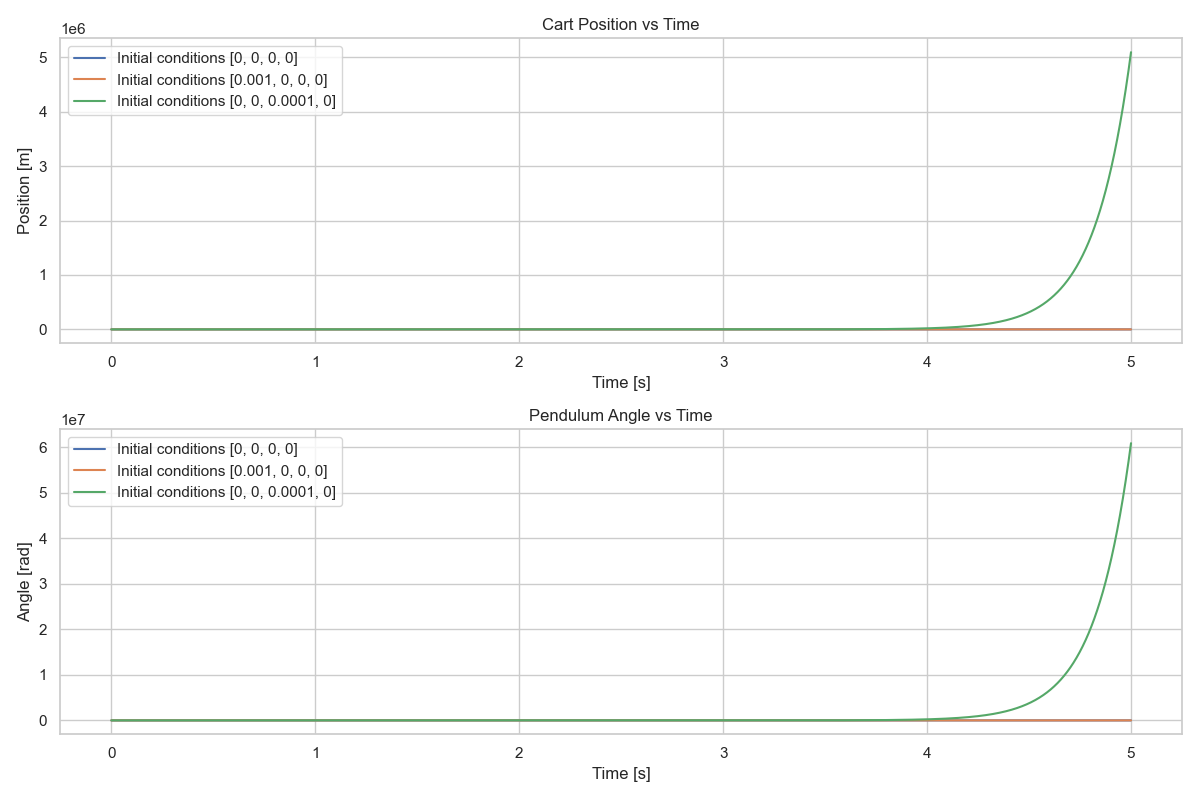
\includegraphics[width=\linewidth]{simulations/system_simulation.png}
\caption{Simulation of the system under different initial conditions. The blue line represents the system starting at a steady state (0,0,0,0). The orange line represents the system with a slight disturbance in velocity (0.001,0,0,0). The green line depicts the system with a disturbance in angle (0,0,0.0001,0).}
\label{fig:system_sim}
\end{figure}

\section{Implementation of LQR Controller}

The LQR gain matrix $K$ is calculated by using the Python Control Systems Library function \texttt{control.lqr}. This function solves the continuous-time Algebraic Riccati equation (CARE) or discrete-time Algebraic Riccati equation (DARE), based on the nature of the system. The function \texttt{control.lqr} requires the state-space model of the system, and the $Q$ and $R$ matrices, as inputs.

With the gain matrix $K$ obtained, the control law $u = -Kx$ is implemented. The control law is used to update the control inputs at each time step in the simulation, which in turn influences the system's state evolution.

Figure \ref{fig:lqr_response} illustrates the response of the system with the LQR controller. As we can see, the LQR controller effectively stabilizes the pendulum in the upright position.

\begin{figure}[h]
\centering
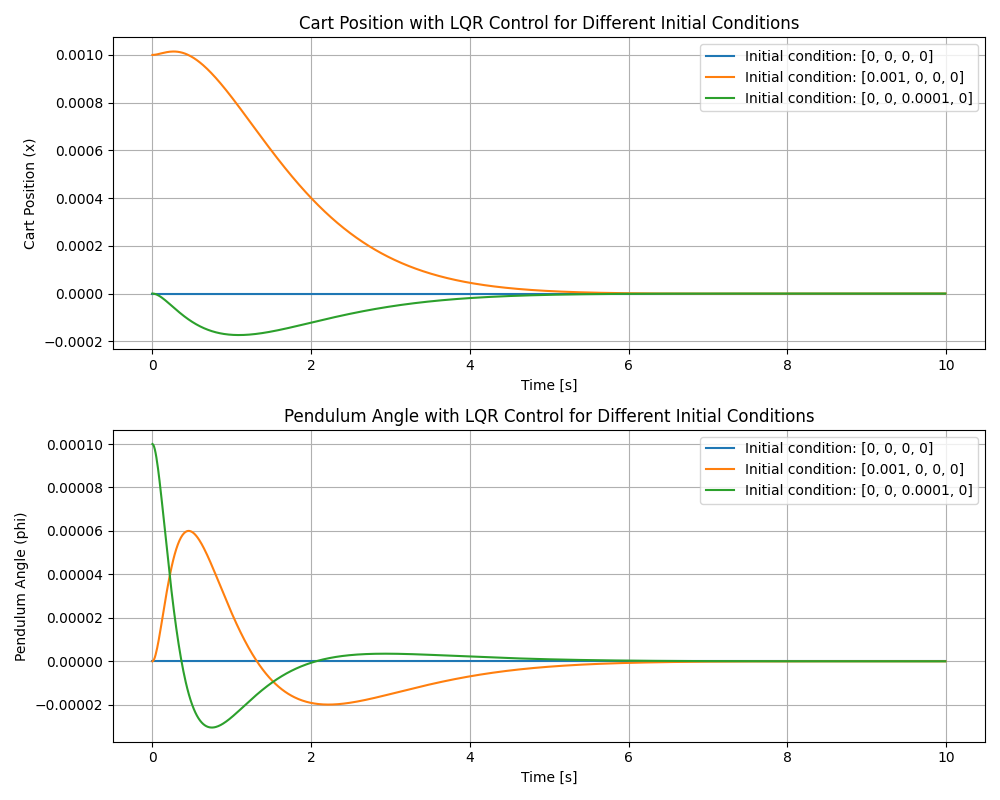
\includegraphics[width=\linewidth]{simulations/lqr_response.png}
\caption{Response of the system under the control of the LQR controller.}
\label{fig:lqr_response}
\end{figure}

The implementation of the LQR controller exhibits its ability to handle multi-input, multi-output (MIMO) systems, while ensuring stability and robustness. It does this by finding the optimal control law that minimizes the cost function, balancing between the control effort and the state deviation. This makes LQR a versatile and powerful controller for a variety of systems.

\section{Exploring Different LQR Parameters}

In LQR controller design, we can adjust the weighting matrices Q and R to emphasize certain control objectives. The matrix Q is used to weigh the states, whereas R is used to weigh the control efforts. 

As a result, changing these matrices affects the control behavior of the system. We performed simulations using high values for elements of the Q matrix (high Q) and high values for elements of the R matrix (high R) to illustrate their impact on system behavior.

\begin{figure}[ht]
    \centering
    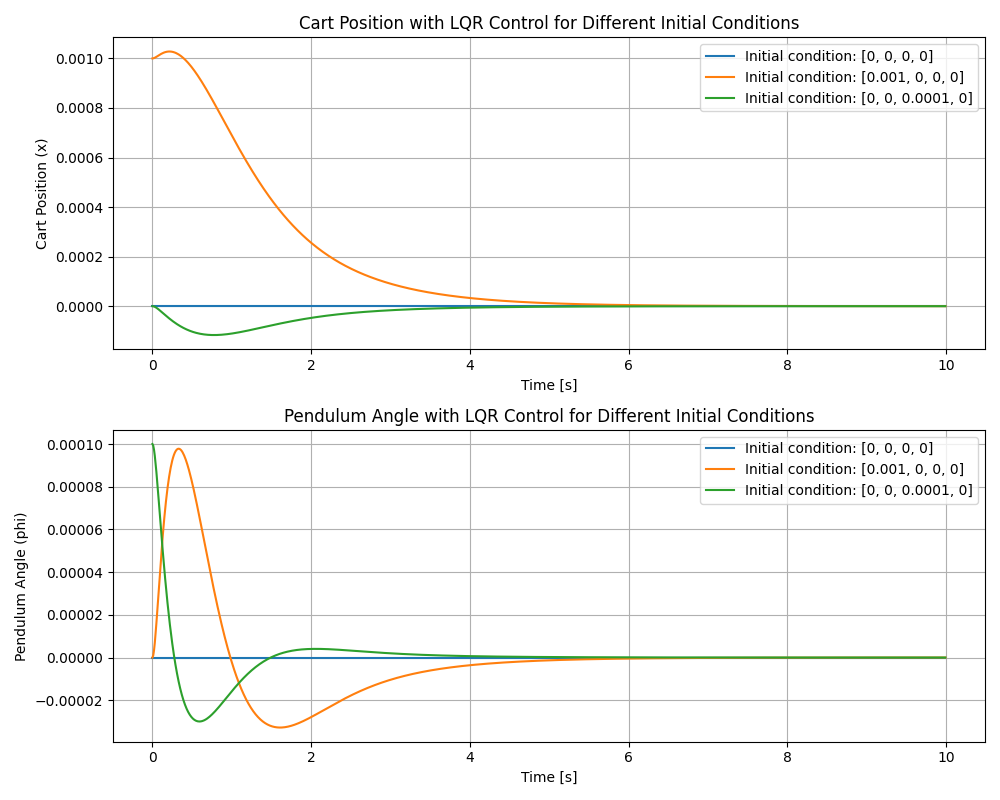
\includegraphics[width=\linewidth]{simulations/high_q_rate.png}
    \caption{System response with high Q. In this case, the states are heavily penalized, and the controller works hard to keep the states near the desired values. This may lead to aggressive control action.}
    \label{fig:high_q}
\end{figure}

\begin{figure}[ht]
    \centering
    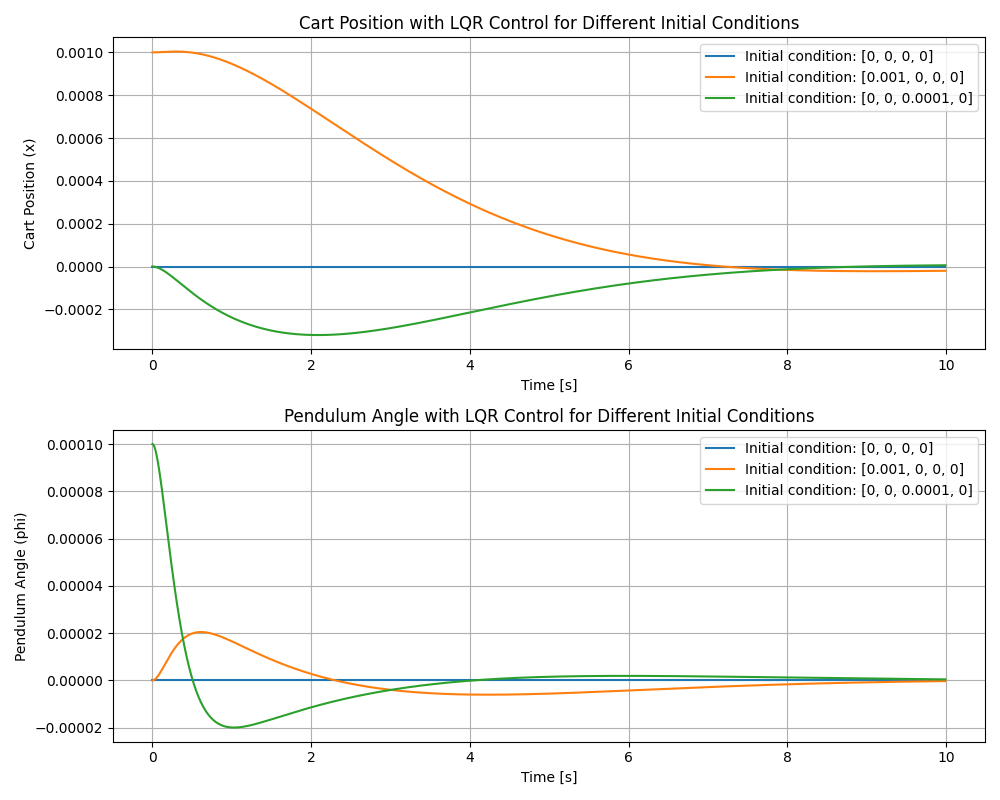
\includegraphics[width=\linewidth]{simulations/high_r_rate.png}
    \caption{System response with high R. In this scenario, the control effort is heavily penalized, and the controller avoids large control actions. This might lead to slower convergence to the desired state, but it also means less energy consumption and less aggressive behavior.}
    \label{fig:high_r}
\end{figure}

As mentioned earlier, changing these matrices affects the control behavior of the system. Here, we explore different LQR parameters and their impact on control effort. Control effort refers to the magnitude of the control signal required to stabilize the system.

\begin{figure}[ht]
    \centering
    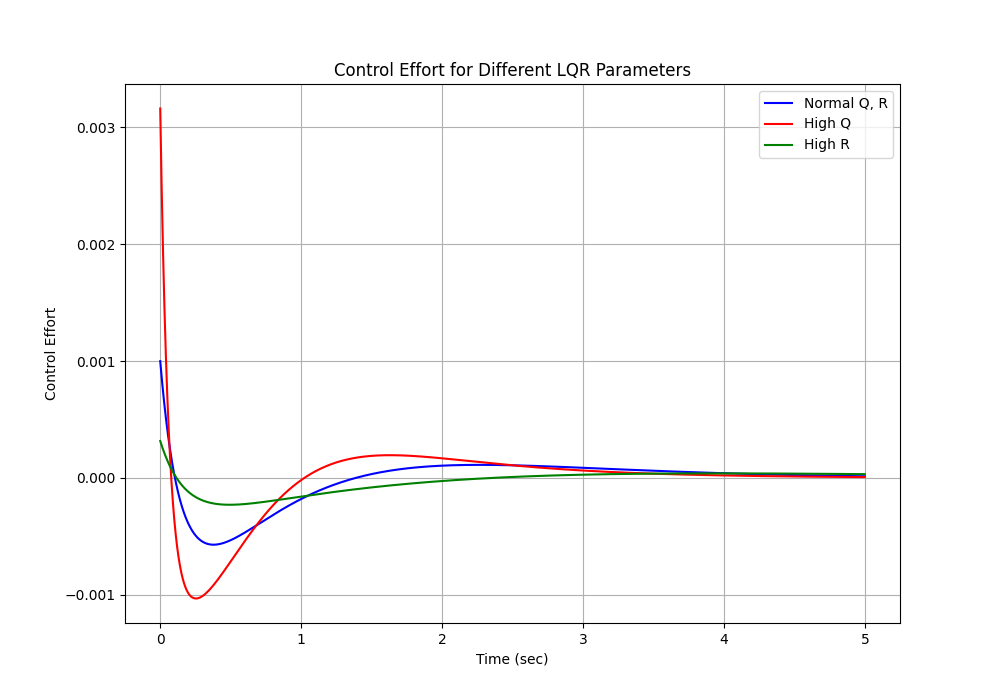
\includegraphics[width=\linewidth]{simulations/control_effort.png}
    \caption{Control effort for different LQR parameters. The blue line represents the control effort with normal Q and R matrices. The red line corresponds to a high Q value, and the green line corresponds to a high R value.}
    \label{fig:control_effort}
\end{figure}

From Figure \ref{fig:control_effort}, we observe that the control effort varies with different LQR parameter settings. A smaller control effort signifies a less aggressive control action, where the controller aims to minimize the energy consumption and reduce large control actions. This can be beneficial in scenarios where excessive control efforts may result in mechanical stress, wear, or undesirable system behavior.

By adjusting the weighting matrices Q and R, we can strike a balance between control effort and system performance. A higher weight on the control effort (higher R value) would lead to smoother control actions at the expense of potentially slower convergence. Conversely, a higher weight on the states (higher Q value) would prioritize reducing the error between the actual and desired states, potentially resulting in more aggressive control actions.

The selection of appropriate LQR parameters depends on the specific system requirements, limitations, and desired trade-offs between performance and control effort. By carefully tuning these parameters, we can achieve the desired control behavior while considering system constraints and optimizing performance.

\subsection{LQR Controller with Varying Cost Matrices}
In this experiment, we implement a Linear Quadratic Regulator (LQR) controller with different weightings for the state and control cost matrices, $Q$ and $R$, respectively. Three scenarios are considered: normal weightings (identity matrices for $Q$ and $R$), increased state cost (ten times the identity for $Q$ and identity for $R$), and increased control cost (identity for $Q$ and ten times the identity for $R$).

The state and control effort of the system are recorded and plotted over a duration of 30 seconds, with setpoints changing at 0s, 10s, and 20s.

\begin{figure}[h]
\centering
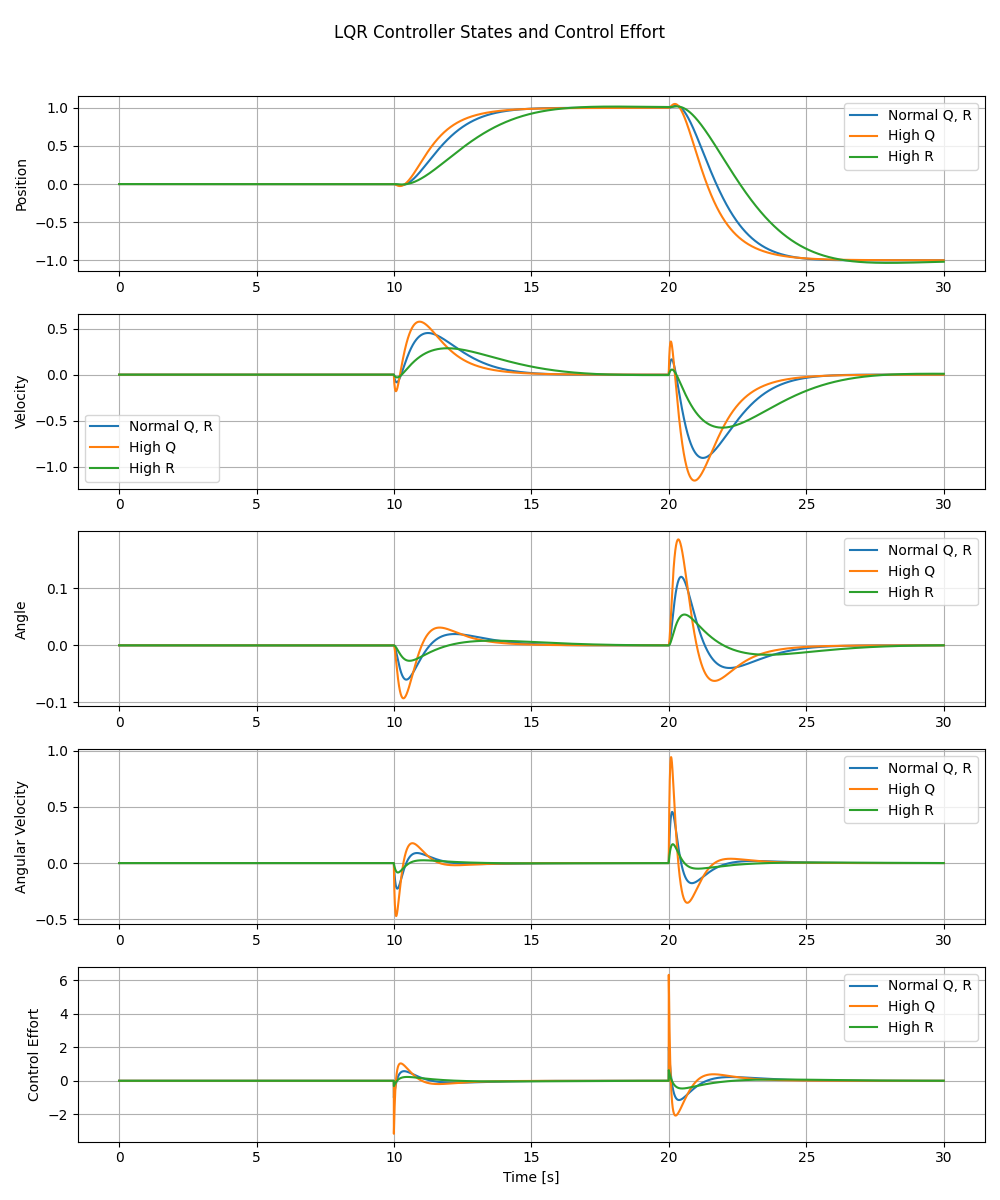
\includegraphics[width=\linewidth]{simulations/lqr_controller.png}
\caption{State and control effort of the LQR controller for normal, high $Q$, and high $R$ cases.}
\end{figure}

The results show that increasing the weighting on the state cost matrix $Q$ results in an increase in control effort. The system responds aggressively to minimize deviations from the setpoint, which can result in high control effort and possibly saturation. Despite the increased control effort, the system does not necessarily reach the setpoint significantly faster.

On the other hand, increasing the weighting on the control cost matrix $R$ results in a more conservative controller that attempts to minimize control effort, possibly at the expense of larger deviations from the setpoint. This might be desirable in scenarios where actuator limitations or energy consumption are of concern.

A further exploration could involve adjusting the weightings in the $Q$ matrix for specific state variables. For instance, what would happen if we heavily weighting the position in the $Q$ matrix while setting other weights to zero?

\subsection{LQR Controller with Varying Cost Matrices and Emphasis on Position}
In the previous experiment, we implemented a Linear Quadratic Regulator (LQR) controller with different weightings for the state and control cost matrices, $Q$ and $R$, respectively. Extending this investigation, we now examine a scenario where the $Q$ matrix is manipulated to assign a significantly higher weight to the positional state, while the weights for other states (velocity, angle, angular velocity) are set to zero. 

This adjustment causes the controller to focus primarily on minimizing positional error, often at the expense of other states. The outcome of this experiment, in terms of state and control effort, is illustrated below.

\begin{figure}[h]
\centering
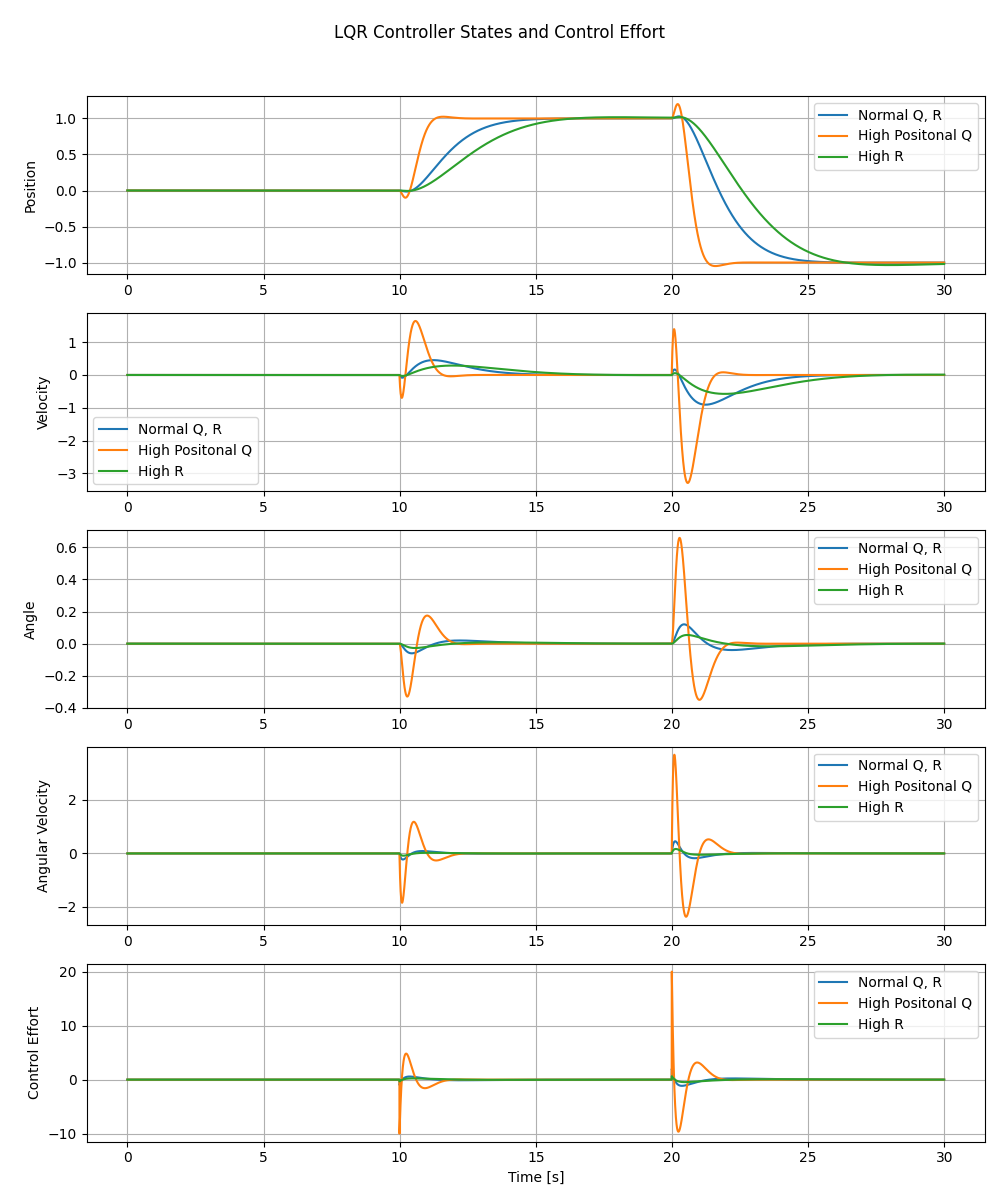
\includegraphics[width=\linewidth]{simulations/lqr_controller_high_posiitonal_q.png}
\caption{State and control effort of the LQR controller with high positional weight in $Q$.}
\end{figure}

As observed from the results, the settling time for position decreases significantly, indicating that the controller is able to reach the positional setpoint much faster than in previous scenarios. However, this comes at the cost of increased deviations in the other state variables. The aggressive control strategy to reduce positional error leads to larger fluctuations in velocity, angle, and angular velocity.

These findings emphasize the trade-off involved in tuning the LQR controller and highlight the flexibility of the LQR framework. By adjusting the weights in the $Q$ and $R$ matrices, the controller's behavior can be tailored to specific requirements. For instance, in scenarios where positional accuracy is of paramount importance, a higher weight can be assigned to the position in the $Q$ matrix, as demonstrated in this experiment. Conversely, if it is crucial to control other state variables more precisely or to limit control effort, the respective weights in the $Q$ and $R$ matrices can be increased.

\section{Conclusion}

This paper provides an in-depth analysis and investigation of the implementation of Linear Quadratic Regulator (LQR) control for a cart-pole system. Various scenarios were examined to better understand the implications of the cost function matrices $Q$ and $R$ on system performance. Our results demonstrated the significant impact of these matrices on both settling time and control effort.

A crucial observation from our experiments was the delicate trade-off between system performance and control effort. It was seen that simply increasing the weights in the $Q$ matrix doesn't necessarily lead to better system response, as it may result in excessive control effort. Therefore, the selection of these weights is an important aspect of designing an LQR controller, and it may require a certain degree of tuning and system knowledge.

Detailed discussion, code, and animations for the results presented in this document \href{https://github.com/sezer-muhammed/LQR-Controller-Examples}{are available in our GitHub repository}. 



\showmatmethods{} % Display the Materials and Methods section
\section{Acknowledgments}

The authors would like to express their gratitude to the \href{https://ctms.engin.umich.edu/CTMS/index.php?example=InvertedPendulum&section=SystemModeling}{University of Michigan's Control Tutorials for MATLAB and Simulink (CTMS)} website for the system model and equations used in this paper. The website served as an invaluable resource, providing a detailed breakdown of the cart-pole system and contributing significantly to our understanding of the Linear Quadratic Regulator control technique implemented in this research.

Special thanks to the contributors of the CTMS website for making the information publicly accessible and promoting a culture of shared learning within the field of control systems.


\showacknow{} % Display the acknowledgments section

% Bibliography
\bibliography{export}


\end{document}